\documentclass[12pt, a4paper, simple]{eskdtext}

\usepackage{hyperref}
\usepackage{_env/gpi_global.env}
\usepackage{_env/gpi_report.env}
\usepackage{_sty/gpi_lst}
\usepackage{_sty/gpi_toc}
\usepackage{_sty/gpi_t}
\usepackage{_sty/gpi_p}
\usepackage{_sty/gpi_u}

% Код
% \ESKDletter{О}{Л}{Р}
% \def \gpiDocTypeNum {81}
% \def \gpiDocVer {00}
% \def \gpiCode {\ESKDtheLetterI\ESKDtheLetterII\ESKDtheLetterIII.\gpiStudentGroupName\gpiStudentGroupNum.\gpiStudentCard-0\gpiDocNum~\gpiDocTypeNum~\gpiDocVer}

\def \gpiDocTopic {Отчёт лабораторной работы №\gpiDocNum}

% Графа 1 (наименование изделия/документа)
% \ESKDcolumnI {\ESKDfontII \gpiTopic \\ \gpiDocTopic}

% Графа 2 (обозначение документа)
% \ESKDsignature {\gpiCode}

% Графа 9 (наименование или различительный индекс предприятия) задает команда
% \ESKDcolumnIX {\gpiDepartment}

% Графа 11 (фамилии лиц, подписывающих документ) задают команды
% \ESKDcolumnXIfI {\gpiStudentSurname}
% \ESKDcolumnXIfII {\gpiTeacherSurname}
% \ESKDcolumnXIfV {\gpiTeacherSurname}

\begin{document}
    \begin{ESKDtitlePage}
    \ESKDstyle{empty}
    \begin{center}
        \gpiMinEdu \\
        \gpiEdu \\
        \gpiKaf \\
    \end{center}

    \vfill

    \begin{center}
        \gpiTopic
    \end{center}

    \vfill

    \begin{center}
        \textbf{\gpiDocTopic} \\
        ПО ДИСЦИПЛИНЕ \gpiDiscipline \\
    \end{center}

    \vfill

    \begin{flushright}
        \begin{minipage}[t]{7cm}
            Выполнил:\\
            \PageTitleStudentInfo
            \PageTitleDateField
            \hspace{0pt}

            Проверил:\\
            \PageTitleTeacherInfo
            \PageTitleDateField
        \end{minipage}
    \end{flushright}

    \vfill

    \begin{center}
        \PageTitleCity~\ESKDtheYear
    \end{center}
\end{ESKDtitlePage}

    \ESKDstyle{empty}
    \begin{center}
        \textbf{\gpiDocTopic}
    \end{center}

    % = = = = = = = =
    \paragraph{} \textbf{Тема}: <<\gpiTopicRep>>

    \paragraph{} \textbf{Цель}:
    приобрести навыки написания простого оконного многопоточного приложения с использованием Java API.

    \paragraph{} \textbf{Что нужно сделать}:

    Разработать оконное приложение с использованием Java API,
    использующее один вспомогательный поток,
    вычисляющий заданную сумму и выполняющий вывод результата вычисления
    (как конечный, так и промежуточные) в любой визуальный компонент.
    Все исходные данные вводятся в соответствующие визуальные компоненты.
    В программе должны быть предусмотрены функции приостановки, возобновления и полной остановки выполнения потока
    с выводом соответствующего сообщения.
    В случае быстрого выполнения потока и, как следствие, невозможности демонстрации функций приостановки,
    продумать искусственное «торможение» потока для достижения заданных целей.
    Обработать исключения.

    \textbf{Вариант 5}:
    $\sum\limits^n_{k=1} = {1 \over {(2k-1)(2k+1)}} = {1 \over 1 * 3} + {1 \over 3 * 5} + ... + {1 \over (2n-1) (2n+1)}$

    \paragraph{} \textbf{Разработка дизайна}:

    % \begin{figure}[!h]
    %     \centering
    %     \includegraphics[]
    %         {_assets/ClassDiagram.png}
    %     \caption{Диграмма классов}
    % \end{figure}

    \begin{figure}[!h]
        \centering
        \begin{minipage}{0.49\textwidth}
            \centering
            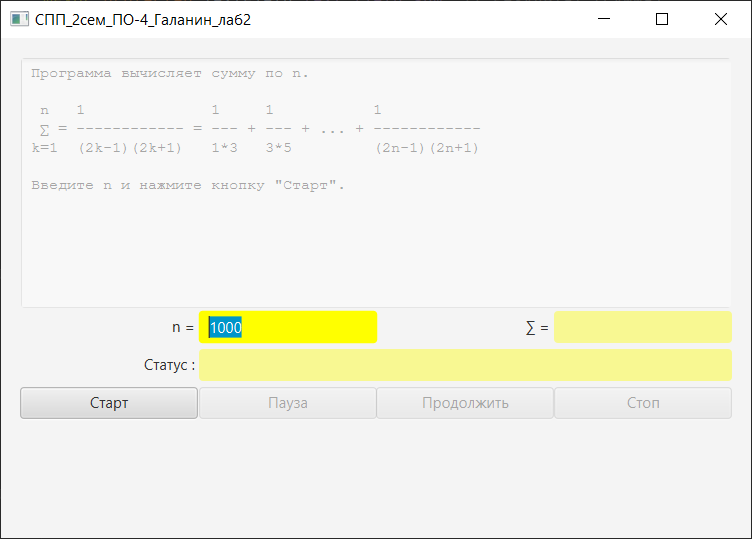
\includegraphics[height=6cm]
                {_assets/input.png}
            \caption{Ввод}
        \end{minipage}
        \begin{minipage}{0.49\textwidth}
            \centering
            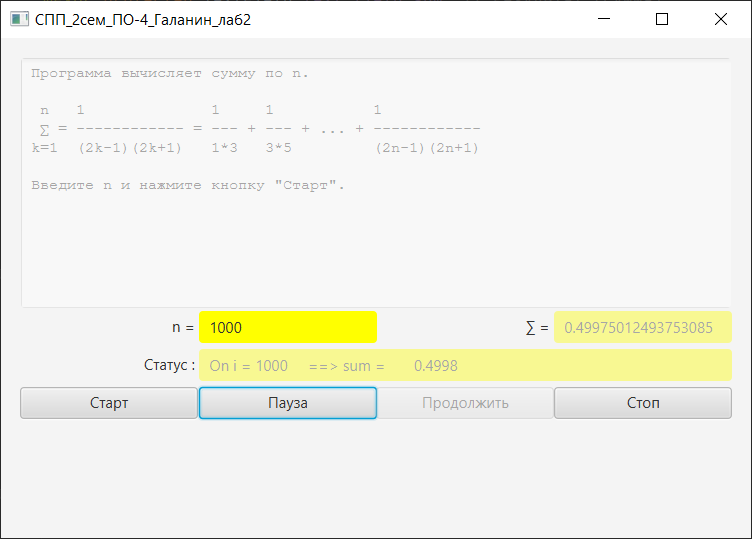
\includegraphics[height=6cm]
                {_assets/output.png}
            \caption{Вывод}
        \end{minipage}
    \end{figure}

    \paragraph{} \textbf{Исходный код}: 

    \begin{itemize}
        \item \textbf{Main.java} - Основная функция программы. Вызывает главное окно.
        \item \textbf{MainApplication.java} - Вызов главного окна. Подключаем дизайн. Задаем заголовок окну.
        \item \textbf{MainController.java} - Контролер клавного окна. Управление кнопок и текстовых полей. Создания потока с таской суммы.
        \item \textbf{CalcTask.java} - Таска расчёта суммы.
        \item \textbf{main-view.fxml} - Дизайн главного окна
    \end{itemize}

    \lstinputlisting[language=java, name=src/main/java/com/example/.../Main.java]
    {../sources/src/main/java/com/example/spp_2sem_po4_galanin_lab2/Main.java}
        
    \lstinputlisting[language=java, name=src/main/java/com/example/.../MainApplication.java]
    {../sources/src/main/java/com/example/spp_2sem_po4_galanin_lab2/MainApplication.java}

    \lstinputlisting[language=java, name=src/main/java/com/example/.../MainController.java]
    {../sources/src/main/java/com/example/spp_2sem_po4_galanin_lab2/MainController.java}

    \newpage
    \lstinputlisting[language=java, name=src/main/java/com/example/.../CalcTask.java]
    {../sources/src/main/java/com/example/spp_2sem_po4_galanin_lab2/CalcTask.java}

    \lstinputlisting[language=xml, name=src/main/resources/com/example/.../main-view.fxml]
    {../sources/src/main/resources/com/example/spp_2sem_po4_galanin_lab2/main-view.fxml}

%     \begin{lstlisting}[caption=Вывод в консоль]
%  Hello, World!
% \end{lstlisting}

    \paragraph{} \textbf{Вывод}:
    Реализовали оконное приложение с многопоточностью:
    основной поток - GUI;
    другой поток - таска, которая вычисляет сумму ряда.
    Реализовали вывод промежуточных результатов в TextEdit (как статус бар).
    Реализовали кнопки старта потока, приастановки и продолжения таски, завершения потока.

    % = = = = = = = =
    % \newpage
    % \addcontentsline{toc}{section}{Список использованных источников}
    % \section*{Список использованных источников}
    \paragraph{} \textbf{Список использованных источников}:
    \begin{enumerate}
        \item[1.] Как создать исполняемый jar файл в IntelliJ IDEA - YouTube [Электронный ресурс]
        - Режим доступа: \url{https://www.youtube.com/watch?v=tA8rEz_xFrQ}.
        Дата~доступа:~01.05.2022.
        \item[2.] Setup IntelliJ IDEA (2021) for JavaFX \& SceneBuilder and Create Your First JavaFX Application - YouTube [Электронный ресурс]
        - Режим доступа: \url{https://www.youtube.com/watch?v=ZfaPMLdgJxQ}.
        Дата~доступа:~01.05.2022.
        \item[3.] JavaFX - Opening an FXML file in New Window - YouTube [Электронный ресурс]
        - Режим доступа: \url{https://www.youtube.com/watch?v=ZzwvQ6pa_tk}.
        Дата~доступа:~01.05.2022.
        \item[4.] How To Fix JavaFX runtime components are missing and are required to run this application - YouTube [Электронный ресурс]
        - Режим доступа: \url{https://www.youtube.com/watch?v=sdkW_cUH3hw}.
        Дата~доступа:~01.05.2022.
        \item[5.] Export JavaFX 11, 15 or 17 projects into an executable jar file with IntelliJ [2022] - YouTube [Электронный ресурс]
        - Режим доступа: \url{https://www.youtube.com/watch?v=F8ahBtXkQzU}.
        Дата~доступа:~01.05.2022.
    \end{enumerate}
    \newpage
\end{document}
